%% FSE (CS-5187 Term Project) research paper. Requirements from the CFP (https://conf.researchr.org/home/fse-2026, checked 2026-09-30):
%%   * \documentclass[acmsmall,screen,review]{acmart}; single column
%%   * deadline: Fri 13 Nov 2026, 23:59 IST
%% Used for e.g. FSE, ISSTA, OOPSLA/PACMPL, TOSEM.
\documentclass[acmsmall,screen,review]{acmart}

%% Shared macros. Keep notation here so the paper cannot drift from itself.
%% Rule: every name, symbol and set used more than once gets a macro here.
\usepackage{amsmath}
\usepackage{booktabs}
\usepackage{xspace}
\usepackage{listings}
\usepackage{xcolor}
\usepackage{array}
\usepackage{pifont}
\usepackage{tikz}
\usetikzlibrary{arrows.meta,positioning,calc,fit,backgrounds}
\DeclareRobustCommand{\circled}[1]{\tikz[baseline=(c.base)]\node[circle,draw,inner sep=0.7pt,font=\tiny\bfseries] (c) {#1};}

% ---- project name ----
% TSCK: the checker's real name, taken directly from its own source
% directory (src/tsck/). Change this one line to rename the tool
% everywhere in the paper; nothing else needs editing.
\newcommand{\tool}{\textsc{Tsck}\xspace}

% ---- notation (one macro per symbol; comment says what it means) ----
% \newcommand{\Seen}[1]{\ensuremath{\mathit{Seen}(#1)}} % example: lines the compiler sees

% ---- research questions ----
\newcommand{\rqref}[1]{\textbf{RQ#1}\xspace}

% ---- results: one boxed, numbered claim per observation ----
\newcounter{observation}
\newsavebox{\obsbox}
\newenvironment{observation}
  {\refstepcounter{observation}\par\smallskip\noindent\begin{lrbox}{\obsbox}\begin{minipage}{0.95\linewidth}\textbf{Observation~\theobservation.}~}
  {\end{minipage}\end{lrbox}\fbox{\usebox{\obsbox}}\par\smallskip}

% ---- CS-5187 term-project FOCUS callouts (RED, on purpose) ----
% A red box that marks a part every term-project report MUST address:
%   Research Questions, Motivating Example, Workflow, Related Work,
%   Threats to Validity. The red is a study aid, not paper style -- once
%   you have written the section, DELETE its \focus{...} line (keep the
%   section). A finished report has zero \focus and zero \todo.
\newcommand{\focus}[1]{%
  \par\smallskip\noindent
  {\color{red}\rule{\linewidth}{0.6pt}}\par\nobreak\vspace{1pt}\noindent
  {\color{red}\ding{228}~\textbf{FOCUS --- graded, must address:}~\itshape #1}\par\nobreak\vspace{1pt}
  {\color{red}\rule{\linewidth}{0.6pt}}\par\smallskip}

% ---- editorial (all must be gone before submission; scripts/check.sh counts them) ----
\newcommand{\todo}[1]{\textcolor{red}{[TODO: #1]}}
\newcommand{\num}[1]{\textcolor{blue}{#1}}   % a number not yet measured by the final tool
\newcommand{\cmark}{\ding{51}}
\newcommand{\xmark}{\ding{55}}

\lstset{basicstyle=\ttfamily\footnotesize,columns=fullflexible,
        keepspaces=true,frame=single,framesep=2pt,xleftmargin=4pt,
        numbers=left,numberstyle=\tiny,numbersep=4pt}

% long \texttt words otherwise run into the margin
\setlength{\emergencystretch}{3em}


\setcopyright{none}
\acmConference[FSE (CS-5187 Term Project)]{ACM International Conference on the Foundations of Software Engineering (Format Template)}{2026}{IIT Guwahati}
\acmYear{2026}
\citestyle{acmauthoryear}

\begin{document}

\title[CVE-Guided Typestate Analysis]{CVE-Guided Typestate Analysis for
  Recurring Vulnerability Detection}


\author{Rutvij Wagh}
\affiliation{\institution{Indian Institute of Technology Guwahati}\country{India}}

\author{Udayraj Choudhary}
\affiliation{\institution{Indian Institute of Technology Guwahati}\country{India}}

\begin{abstract}
A public vulnerability fix teaches a lifecycle rule: an object must not
be released without resetting a caller-visible reference to it, or
without detaching it from a chain it still belongs to. Existing
general-purpose static analyzers do not check a specific project's own
such conventions; they check their own stock rule sets instead.
CVE-2022-4450 is a real case: \texttt{PEM\_read\_bio\_ex} in OpenSSL frees
two output buffers on one failure path without clearing the
caller-visible pointers to them, letting a caller double-free. We present
\tool, which reads such a rule from a data file and checks it against a
\texttt{tree-sitter} control-flow graph. On OpenSSL, \tool flags \texttt{PEM\_read\_bio\_ex}'s two outputs
before the fix and clears both after it. It also reproduces an unrelated
non-CVE fix the rule was never shown, and flags one site a later OpenSSL
commit went on to fix independently.
On the current 1{,}155-file \texttt{crypto/ssl/providers} tree it flags
10 sites: manual triage finds 2 potential recurrences whose failure
branch is not reachable in normal builds, 8 harmless deviations, and 0
confirmed new vulnerabilities. None of three
general-purpose open-source static analyzers we ran, with their stock
configuration, distinguishes any of three historical CVEs from their own
fix; a project-specific rule, not a sharper general one, closed that gap.
A second, differently-shaped rule for the detach-before-release BIO-chain
invariant behind CVE-2023-0215 reuses the same parser and control-flow
graph and also distinguishes its own motivating fix. Its whole-tree run,
though, flags 11 sites that are all false positives, because the rule has
no notion of which released object is externally owned. 

\end{abstract}

%% CCS concepts: pick the ones that fit YOUR project at https://dl.acm.org/ccs
%% (500 = main, 300 = secondary). This template fits any software-engineering
%% topic -- static analysis, dynamic analysis/testing, empirical studies,
%% program repair, tools, human factors, etc. -- so replace the placeholder
%% below with the concept for your own work. A few common top-level ids:
%%   Software and its engineering~Software testing and debugging
%%   Software and its engineering~Automated static analysis
%%   Software and its engineering~Dynamic analysis
%%   Software and its engineering~Software creation and management
%%   General and reference~Empirical studies
%% TODO (authors, not Claude): the concept_id digits below are a best guess,
%% not independently verified against the live generator -- it is only
%% reachable at https://dl.acm.org/ccs, not fetchable from this session.
%% Before submission, regenerate this exact block from that tool by
%% selecting "Software and its engineering > Automated static analysis" and
%% "Security and privacy > Software and application security" (or whichever
%% leaf concepts best fit) and paste its output here verbatim.
\begin{CCSXML}
<ccs2012>
  <concept>
    <concept_id>10011007.10011074.10011099</concept_id>
    <concept_desc>Software and its engineering~Automated static analysis</concept_desc>
    <concept_significance>500</concept_significance>
  </concept>
  <concept>
    <concept_id>10002978.10002991</concept_id>
    <concept_desc>Security and privacy~Software and application security</concept_desc>
    <concept_significance>300</concept_significance>
  </concept>
</ccs2012>
\end{CCSXML}
\ccsdesc[500]{Software and its engineering~Automated static analysis}
\ccsdesc[300]{Security and privacy~Software and application security}

\keywords{static analysis, typestate analysis, control-flow graph,
  recurring vulnerabilities, OpenSSL, memory safety, output parameters,
  tree-sitter}

\maketitle

\section{Introduction}
\label{sec:intro}

Suppose you have just read a public vulnerability fix for a C library you
depend on: a one-line patch that frees a buffer and then clears the
pointer to it, because the code path that frees it can be reached again
before the function returns. You trust the fix. The natural next question
is whether the same mistake, the same missing reset after the same kind
of release, sits somewhere else in the same codebase, in a function the
patch never touched.

Static analyzers already look for memory-safety bugs in C, and some are
free and widely used: Clang Static Analyzer, Cppcheck, and Coccinelle
semantic patches, among others. These tools ship with general rule sets
built from common bug patterns across many projects. They stop short of
one thing: a rule derived from a single project's own patch history, for
the exact ownership or reset convention that patch teaches, checked
everywhere that convention should hold in that project's current source.

We focus on a second problem that starts where general-purpose rule sets
stop. Given one historical fix, can a rule extracted from it, with no
function names baked in, be checked against a project's whole source
tree? We ask three things of such a rule: (i)~flag the function the fix
came from before the fix, and clear it after; (ii)~do the same for an
unrelated fix nobody built the rule from; and (iii)~say, for every site it
flags on the project's current source, whether that site is conforming, a
real violation, or explainable, with a witness a human can check by hand.

CVE-2022-4450~\cite{nvd2022cve4450} is a real case. \texttt{PEM\_read\_bio\_ex} in OpenSSL's
\texttt{crypto/pem/pem\_lib.c} frees two output buffers on one failure
path (Figure~\ref{fig:motivating}) without clearing the caller-visible
pointers to them; a caller that frees these outputs again after failure
can double-free. The fix, commit \texttt{63bcf189be}, adds exactly two
assignments.

Closest to our rule-as-data approach is VulPA~\cite{cao2025vulpa}, which
also derives a checkable rule from a known bug, but compiles it to an
automaton checked by an interprocedural analysis with aliasing, on Java.
Ours is intraprocedural, with no alias analysis (Section~\ref{sec:related}).

We present \tool, a checker that reads a lifecycle rule from a data file
and applies it to real C source through a parser and a per-function
control-flow graph built with \texttt{tree-sitter}, searches for a path
from each release of an output parameter to function exit that never
resets it, and classifies each site with a witness path
(Section~\ref{sec:approach}). This paper implements two such rules against the same parser and CFG
builder: Protocol~B, for the output-pointer reset convention behind
CVE-2022-4450, and Protocol~A, for the detach-before-release BIO-chain
convention behind CVE-2023-0215~\cite{nvd2023cve0215} (\rqref{5}, Section~\ref{sec:rq5}).

On OpenSSL, \tool flags \texttt{PEM\_read\_bio\_ex}'s two output
parameters before the fix and clears both after it. It also reproduces an
unrelated non-CVE fix the rule was never shown, and flags one site a
later OpenSSL commit went on to fix independently
(Section~\ref{sec:eval}). On the current source tree it flags 10 sites.
Manual triage finds 2 potential recurrences whose failure branch is not
reachable in normal builds, 8 harmless deviations, and 0
confirmed new vulnerabilities. The lesson we did not expect going in:
none of three general-purpose open-source static analyzers, run with
their stock configuration, distinguishes any of the three CVEs we
checked from its own fix (Section~\ref{sec:rq2}). A project-specific
rule, not a sharper general one, is what closed the gap here. Protocol~A
also distinguishes its own motivating fix, but its whole-tree run finds
0 confirmed recurrences out of 11 flagged sites, all false positives from
the rule's missing notion of object ownership: the rule-as-data
architecture generalizes across invariant shapes even where a given
rule's detection does not generalize across a whole codebase
(Section~\ref{sec:rq5}).

\paragraph{Contributions.} (1)~A rule-as-data lifecycle invariant for
output-pointer reset after release, independent of any function name
(Section~\ref{sec:problem}); (2)~\tool, which checks it on a real
\texttt{tree-sitter} control-flow graph (Section~\ref{sec:approach});
(3)~an evaluation on six pinned OpenSSL snapshots and a four-tool
comparison on three historical CVEs (Section~\ref{sec:eval}); (4)~a second,
differently-shaped rule, Protocol~A, showing where single-object
generalization breaks down (Section~\ref{sec:rq5}); and (5)~the released
tool and data (Section~\ref{sec:data}).

\begin{figure}[t]
\begin{lstlisting}[numbers=none,escapechar=@]
headerlen = BIO_get_mem_data(headerB, NULL);
*header = pem_malloc(headerlen + 1, flags);
*data = pem_malloc(len, flags);
if (*header == NULL || *data == NULL)
    goto out_free;
...
out_free: @\textcolor{red}{// *header, *data freed, never reset}@
    pem_free(*header, flags, 0);
    pem_free(*data, flags, 0);
end:
    ...
    return ret; @\textcolor{red}{// caller sees stale *header, *data}@
\end{lstlisting}
\caption{\texttt{PEM\_read\_bio\_ex} in OpenSSL \texttt{8e257b86e5}
  (\texttt{crypto/pem/pem\_lib.c}, trimmed). The \texttt{out\_free} path
  frees \texttt{*header} and \texttt{*data} but never resets either
  pointer before \texttt{return}. The fix, commit \texttt{63bcf189be},
  adds \texttt{*header = NULL;} and \texttt{*data = NULL;} to this path.}
\label{fig:motivating}
\Description{Code excerpt from OpenSSL showing two output pointers freed on an error path without being reset to null before the function returns.}
\end{figure}

\section{Background}
\label{sec:background}

\paragraph{Output parameter.} A C function can return a value through a
parameter of pointer-to-pointer type, written \texttt{T **P}. The caller
passes the address of its own pointer variable; the function writes a
value into \texttt{*P} for the caller to read after the call returns. We
write \texttt{*P} for the object the caller's pointer refers to, not for
\texttt{P} itself.

\paragraph{Release and reset.} A \emph{release} of \texttt{*P} is a call
that frees the object \texttt{*P} points to, for example
\texttt{OPENSSL\_free(*P)}. After a release, \texttt{*P} still holds the
freed address unless something changes it. A \emph{reset} of \texttt{*P}
is an assignment that gives it a new value, most often \texttt{*P = NULL}.
A dangling \texttt{*P}, one that still holds a freed address after a
release and before any reset, is dangerous exactly when the caller can
read or free it again: a double free, or a use of freed memory if the
caller dereferences it.

\paragraph{Typestate.} \emph{Typestate analysis} tracks not just an
object's type but which operations are currently valid on it, as a small
state machine. \todo{Cite the originating typestate paper once its
author list and venue are verified directly (for example on IEEE Xplore);
automated search returned conflicting author lists for this title across
mirrors and we do not cite it unverified.} For the invariant in this paper,
\texttt{*P} moves through three states: \emph{Valid} before any release,
\emph{Released} after a release and before a reset, and back to
\emph{Valid} (we call it \emph{Reset}, to keep the release that caused it
visible in our output) once a reset occurs. A \emph{violation} is a
program path on which \texttt{*P} can reach function exit while still in
the \emph{Released} state. CVE-2022-4450 (Section~\ref{sec:rq1}) is
exactly this: \texttt{PEM\_read\_bio\_ex} frees \texttt{*header} and
\texttt{*data} on one failure path and returns without resetting either.

\paragraph{Release site.} We call the specific call expression that
performs a release, together with its source location and the parameter
\texttt{P} it releases, a \emph{release site}. Section~\ref{sec:eval}
reports counts of release sites, not of functions: one function can
contain several release sites, one per output parameter it releases.

\paragraph{Rule as data.} Existing patch-matching checkers, including the
Part~1 baseline in this project (\texttt{typestate\_check.py}), encode a
rule as a sequence of string or syntax checks written for one named
function. We instead write the rule once as data
(Section~\ref{sec:rule}), independent of any function name, and apply it
to every function in a source tree that has a parameter of the tracked
shape.

%% Optional pilot section intentionally excluded from main.tex. The project
% does not preserve a separate pre-tool pilot measurement with a counting
% definition and raw data that can be reported independently of the final
% evaluation. The final paper therefore reports the measured evaluations
% in Section~\ref{sec:eval} instead of presenting an unsupported pilot.
          % optional: "A First Look" before the tool
\section{Problem Statement}
\label{sec:problem}

We now state the problem precisely. Let $f$ be a C function with a
parameter $P$ of pointer-to-pointer type or deeper. Let $r$ be a
\emph{release site} inside $f$: a call that frees the object $*P$ points
to (Section~\ref{sec:background}). A \emph{reset} of $*P$ is an assignment
to $*P$, or, when the rule allows it, passing $P$ itself to a call that
may reassign it. Let $\mathrm{paths}(r)$ be the set of control-flow paths
from $r$ to the exit of $f$, built from $f$'s real parse tree
(Section~\ref{sec:step1}).

\paragraph{Goal.} $r$ is \emph{conforming} if every path in
$\mathrm{paths}(r)$ passes a reset of $*P$ before reaching exit. $r$ is a
\emph{violation} if some path in $\mathrm{paths}(r)$ reaches exit without
passing a reset. Given a rule (Section~\ref{sec:rule}) and a C source
tree, our goal is to compute this conforming/violation label, with a
witness path, for every release site whose parameter matches the rule.

\paragraph{Why not grep for the release/reset pair?} A regular expression,
like the Part~1 baseline \texttt{typestate\_check.py}, can check that a
function's text contains both a release and a reset. It cannot tell
whether the reset lies on \emph{every} path from the release to exit or on
only one branch, nor distinguish a reset in dead code; that needs a parse
tree and a control-flow graph.

\section{Approach}
\label{sec:approach}

Figure~\ref{fig:overview} shows the steps of \tool. The main idea is to
read a lifecycle rule from a data file, rather than hard-coding it. \tool
checks that rule against a per-function control-flow graph built from the
real parse tree of each C source file. This paper implements two such
rules against the same parser and CFG builder: Protocol B
(Section~\ref{sec:step2}), a release/reset rule derived from
CVE-2022-4450, and Protocol A (Section~\ref{sec:rq5}), a differently-shaped
establish/detach-before-release rule for the BIO-chain invariant behind
CVE-2023-0215. We return to what each rule does and does not generalize
to in Section~\ref{sec:threats}.

\begin{figure}[t]
  \centering
  %% Figure: overview of \tool (Protocol B). Steps left to right; the dashed
%% back-edge is the outer loop over pinned OpenSSL snapshots in run_scan.sh,
%% not an iteration inside one file's analysis.
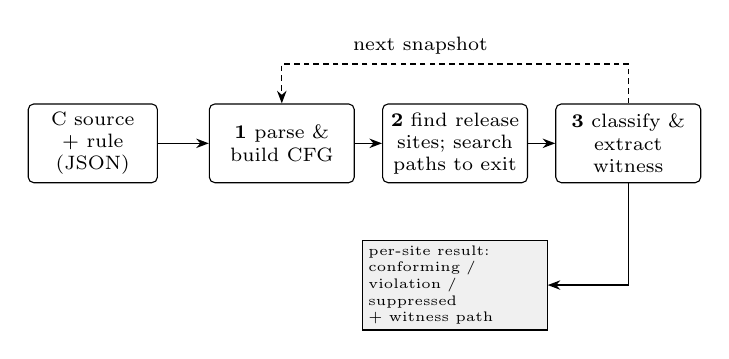
\begin{tikzpicture}[
    x=1cm, y=1cm, font=\scriptsize,
    box/.style={draw, rounded corners=2pt, align=center, inner sep=2pt,
                minimum height=10mm, text width=17mm, fill=white},
    outbox/.style={draw, align=left, inner sep=2pt, fill=black!6,
                text width=22mm, font=\tiny},
    flow/.style={-{Stealth[length=1.6mm]}, line width=0.5pt},
    back/.style={-{Stealth[length=1.6mm]}, line width=0.5pt, dash pattern=on 2pt off 1.5pt},
  ]
  \node[box, text width=15mm] (in) at (-0.3,0) {C source\\+ rule (JSON)};
  \node[box] (s1) at (2.1,0) {\textbf{1} parse \&\\ build CFG};
  \node[box] (s2) at (4.3,0) {\textbf{2} find release\\ sites; search\\ paths to exit};
  \node[box] (s3) at (6.5,0) {\textbf{3} classify \&\\ extract witness};
  \node[outbox] (o) at (4.3,-1.8) {per-site result:\\ conforming /\\ violation /\\ suppressed\\ + witness path};
  \draw[flow] (in) -- (s1);
  \draw[flow] (s1) -- (s2);
  \draw[flow] (s2) -- (s3);
  \draw[flow] (s3.south) |- (o.east);
  \draw[back] (s3.north) -- ++(0,0.5) -| node[pos=0.3, above] {next snapshot} (s1.north);
\end{tikzpicture}

  \caption{\tool takes a C source tree and a rule stored as data
    (Section~\ref{sec:rule}). It parses every file once, finds every site
    that releases a tracked pointer, and searches forward in the
    control-flow graph for a path to function exit that never resets it.
    Each flagged site keeps a witness path. The outer loop (dashed) reruns
    this per pinned OpenSSL snapshot; nothing loops within one file's
    analysis.}
  \label{fig:overview}
\end{figure}

\subsection{The rule, as data}
\label{sec:rule}
The rule for Protocol B is a JSON file, not a code path: it names no
OpenSSL function. It tracks parameters of pointer-to-pointer type; a
\emph{release} is any call whose name matches the regular expression
\texttt{(?i)free} and whose argument is \texttt{*P}; a \emph{reset} is an
assignment to \texttt{*P}, or, by a configurable flag, passing \texttt{P}
itself to a later call. The invariant is: if a function releases
\texttt{*P}, every path from that release to function exit must reach a
reset first. We do not claim the idea of an output-parameter reset
invariant as new; what we built is a parser and path-search engine that
checks it against real source, rather than against one patch's text.

\subsection{Step 1: Parsing and the control-flow graph}
\label{sec:step1}
\tool parses each C file with \texttt{tree-sitter} and
\texttt{tree-sitter-c}. We do not claim parsing itself as new; everything
from here on is. For each function, we build a control-flow graph whose
nodes are simple statements, branch and loop conditions, labels, and join
points; \texttt{goto} targets, including error labels such as
\texttt{err:}, become real edges, so an error path that jumps past a reset
is visible to the path search in Step~2. Three approximations keep the
graph tractable and are stated as threats to validity
(Section~\ref{sec:threats}): a compound condition joined by \texttt{\&\&}
or \texttt{||} is one node, without separate short-circuit edges; a
\texttt{\#if}/\texttt{\#ifdef} block is treated as a branch, keeping both
variants rather than resolving the macro; and macro bodies are not
expanded, so a macro call is treated as an ordinary call expression.

\subsection{Step 2: Release sites and the path search}
\label{sec:step2}
For every parameter \texttt{P} of pointer-to-pointer type or deeper, \tool
scans each control-flow node for calls matching the release pattern and
for assignments matching the reset pattern. From every release site, it
searches the control-flow graph forward, breadth-first, for a path to
function exit. The search stops following a branch once it crosses a
reset, and the release's own dereference of \texttt{*P} licenses one
pruning rule: because the release itself has already dereferenced
\texttt{*P}, \texttt{P} is non-null on every path after it, so a later
branch that is live only when \texttt{P == NULL} is dead code and is not
explored. If the search reaches function exit without crossing a reset,
the site is a candidate violation and the path taken becomes its witness.

Two refinements narrow this candidate set. We disclose both as chosen
after reading real output, not derived from the rule alone. \emph{Deref-
after-release suppression} drops a site where \texttt{*P} is read again
before any reset. This signals a partial release and reuse, not a
dangling pointer: for example, a function that frees only part of a
struct's contents and then reinitializes it. The second refinement is the
\texttt{NULL}-guard pruning described above, added after it produced one
infeasible-path false positive on a whole-tree scan. Both are unit-tested
(Section~\ref{sec:eval}) and are listed, not hidden, in each result.

\subsection{Step 3: Classification and witness extraction}
\label{sec:step3}
Each release site is labeled \emph{conforming} if every path from it to
function exit passes a reset; \emph{violation} if some path reaches exit
without one; or \emph{suppressed} if the path rule would flag it but one
of the two refinements in Step~2 applies. A suppressed site is reported,
with its reason, alongside conforming and violation sites; it is never
dropped silently. For a violation, \tool records the source lines on the
witness path. A reader can then check the finding against the source
without re-running the tool. \texttt{compare.py} diffs two runs of the
same files at different revisions and reports exactly which sites a given
commit removed or added. Section~\ref{sec:eval} uses this to measure
whether a real fix changes only the sites its own diff touches.

%% Optional section. It is excluded from main.tex to preserve the current
% paper structure and page budget. The content below is a concise record of
% the implementation and can be included if the authors need this detail.
\section{Implementation}
\label{sec:impl}

The prototype is written in Python. It uses the Tree-sitter C grammar to
parse source files and builds a control-flow graph for each function that
contains a parameter matching the selected rule. The graph represents
branching and loop structure so that the checker can search paths from a
lifecycle event to function exit.

Protocol~B is implemented in \texttt{outparam.py} and configured by
\texttt{specs/outparam\_reset.json}. It tracks release and reset events
for pointer-to-pointer parameters. Protocol~A is implemented in
\texttt{protocol\_a.py} and configured by
\texttt{specs/bio\_chain\_pop.json}. It tracks BIO-chain establishment,
detachment, and release events. Both rules reuse the parser and CFG
builder; their event specifications and path checks differ.

The repository includes unit and regression tests for the analysis
engine and the two protocols. The shell scripts in \texttt{src/tsck/}
run the pinned OpenSSL scans and preserve their logs and machine-readable
results. The final paper does not include this optional section; the
reproducibility details are summarized in Section~\ref{sec:data}.
 % optional
\section{Evaluation}
\label{sec:eval}

We ask five questions.
\begin{itemize}
  \item[\rqref{1}] Does \tool (the invariant-based Protocol B engine) detect
    the motivating CVE on real OpenSSL source, distinguish the fix from the
    bug, and generalize to a fix it was not derived from?
  \item[\rqref{2}] Do general-purpose open-source static-analysis tools
    already catch the bugs a source-pattern baseline catches, on the same
    three CVEs?
  \item[\rqref{3}] Does a rule written from one CVE flag a site that
    OpenSSL fixed only later, without the rule being changed after the
    fact?
  \item[\rqref{4}] What does \tool cost in time?
  \item[\rqref{5}] Does \tool's rule-as-data design extend to a second,
    differently-shaped invariant (Protocol A, CVE-2023-0215), and does that
    second rule generalize the same way Protocol B's did?
\end{itemize}

\subsection{Subjects}
\label{sec:subjects}
We select three historical OpenSSL CVEs and one non-CVE fix, each a pinned
vulnerable/fixed commit pair with a publicly documented root cause (so the
label is not our judgment), source at both revisions in the same file, and
at least one case not used to derive the rule (\rqref{3}).
CVE-2022-4450 (\texttt{PEM\_read\_bio\_ex}, fix \texttt{63bcf189be}) is the
source of Protocol~B. CVE-2023-0215 (\texttt{BIO\_new\_NDEF}, fix
\texttt{8818064ce3}) is the second baseline CVE (\rqref{2}) and the source
of Protocol~A (\rqref{5}). CVE-2024-4741 (\texttt{SSL\_free\_buffers}, fix
\texttt{b3f0eb0a29}) is in the baseline comparison only: it needs a state
guard neither rule can express, and we report that scope rather than drop
the case. The \texttt{d2217c88df} KDF fix (not a CVE, a different author, a
year before CVE-2022-4450) is the out-of-sample case.

\subsection{Baselines}
\label{sec:baselines}
The \emph{Part~1 pattern baseline} is \texttt{typestate\_check.py}, the
project's own string/regex patch matcher, included as the simplest thing
that could work. \emph{Clang Static Analyzer~18} ran via
\texttt{scan-build-18} on each revision's affected translation unit with its
generated build flags. \emph{Coccinelle~1.1.1} ran five pre-existing
semantic patches (not written for these CVEs) for release/use, repeated
release, release-after-transfer, and allocate-then-return.
\emph{Cppcheck~2.13.0} ran with \texttt{--enable=warning,style,performance,
portability --inconclusive} (C11/unix64). None was tuned toward these
CVEs. Because Protocol~B has no rule for two of the three CVEs, this
compares general tools against the baseline, not against \tool. For each
tool and revision we manually read whether the output distinguishes
vulnerable from fixed.

\subsection{Setup}
\label{sec:setup}
\tool (Protocol~B) ran on Python~3.13, \texttt{tree-sitter}~0.26.0,
\texttt{tree-sitter-c}~0.24.2 (Linux, WSL2). The \rqref{2} baselines ran on
a separate machine (Python~3.12.3, Clang~18.1.3, Coccinelle~1.1.1 on
OCaml~4.14.1, Cppcheck~2.13.0); executable hashes and frozen rule files are
recorded with the data, and no measurement mixes the two environments. For
\rqref{4}, a second author reran \texttt{run\_scan.sh} on a third machine
(Python~3.11.6, same \texttt{tree-sitter} versions) under
\texttt{/usr/bin/time -v}. Protocol~A's runs (\rqref{5}) were reproduced on
a fourth environment (\texttt{tree-sitter}~0.26.1) with identical counts.

\subsection{\rqref{1}: Does \tool detect and generalize the motivating CVE?}
\label{sec:rq1}

\begin{table}[t]
  \centering
  \caption{\tool (Protocol B) on six pinned OpenSSL snapshots
    (\texttt{crypto/}, \texttt{ssl/}, \texttt{providers/}). A
    \emph{release site} is a call that frees \texttt{*P} for a
    pointer-to-pointer parameter \texttt{P}. The two fixes each remove
    exactly their own violations and add none.}
  \label{tab:rq1-wholetree}
  \begin{tabular}{lrrrr}
    \toprule
    Snapshot & C files & Conforming & Violation & Suppressed \\
    \midrule
    CVE-2022-4450 pre-fix (\texttt{8e257b86e5})  & 1001 & 99  & 7  & 2 \\
    CVE-2022-4450 fix (\texttt{63bcf189be})      & 1001 & 101 & 5  & 2 \\
    KDF fix parent (\texttt{29a27cb2c5})         & 1005 & 93  & 12 & 2 \\
    KDF fix (\texttt{d2217c88df}, not a CVE)     & 1005 & 97  & 8  & 2 \\
    OpenSSL 3.0.0 (\texttt{89cd17a031})          & 999  & 92  & 10 & 2 \\
    master (\texttt{949fe8b5f4}, 2026-10-30)     & 1155 & 132 & 10 & 2 \\
    \bottomrule
  \end{tabular}
\end{table}

Table~\ref{tab:rq1-wholetree} shows \tool on the motivating function and on
the whole tree. At the vulnerable revision, \tool flags
\texttt{PEM\_read\_bio\_ex}'s \texttt{*header} and \texttt{*data} as
violations (witness lines 991--998); at the fix, both sites are
conforming. The same fix removes exactly these two violations from the
whole-tree count (99~$\to$~101 conforming, 7~$\to$~5 violation) and adds
none.

\begin{observation}
\label{obs:rq1-conformance}
\tool is not limited to the function it was derived from: the unrelated,
non-CVE \texttt{d2217c88df} KDF fix removes exactly the four violations
its own commit changes (\texttt{pbkdf1}, \texttt{pbkdf2}, \texttt{pkcs12kdf},
\texttt{scrypt}, each \texttt{*buffer}) and adds none, with the rule
unchanged from the CVE-2022-4450 derivation.
\end{observation}

\begin{observation}
\label{obs:rq1-mastertriage}
On current master, \tool flags 10 sites; manual triage against each site's
callers found 2 potential recurrences whose failure branch is not
reachable in normal builds, 8 convention deviations with no caller impact,
and 0 confirmed new vulnerabilities. (Two of the eight were initially
labelled "unclear" pending a caller read; Section~\ref{sec:threats}
reports that re-check.) We report this plainly: the contribution here is
a bounded rule that reproduces two real fixes without retuning, not a new
bug.
\end{observation}

\subsection{\rqref{2}: Do general-purpose tools already catch these bugs?}
\label{sec:rq2}

\begin{table}[t]
  \centering
  \caption{Detection on the vulnerable/fixed pair for each CVE: whether
    the tool's output distinguishes the two revisions for the
    CVE's own mechanism. \cmark{} = distinguishes vulnerable from fixed;
    \xmark{} = does not. The Part 1 pattern baseline is not \tool; see
    Section~\ref{sec:baselines}.}
  \label{tab:rq2-comparison}
  \begin{tabular}{@{}lccc@{}}
    \toprule
    Tool & \shortstack{2022\\4450} & \shortstack{2023\\0215} & \shortstack{2024\\4741} \\
    \midrule
    Part 1 pattern baseline & \cmark & \cmark & \xmark$^{a}$ \\
    Clang Static Analyzer~18 & \xmark & \xmark & \xmark \\
    Coccinelle~1.1.1 & \xmark & \xmark & \xmark \\
    Cppcheck~2.13.0 & \xmark & \xmark & \xmark \\
    \bottomrule
  \end{tabular}
\end{table}

The columns correspond to CVE-2022-4450~\cite{nvd2022cve4450},
CVE-2023-0215~\cite{nvd2023cve0215}, and
CVE-2024-4741~\cite{nvd2024cve4741}, respectively. $^{a}$On the
corrected CVE-2024-4741 pair (\texttt{ec559c2a6c}/\texttt{b3f0eb0a29}) the
Part~1 baseline alerts on both sides; it is quiet only on the later hardening
commit \texttt{2d05959073}, so it matches that pattern, not the advisory's
state-guard fix.
Table~\ref{tab:rq2-comparison} compares four tools on six pinned revisions
(three CVEs, vulnerable and fixed side). A Clang positive control, run on a
synthetic use-after-free, produced the expected diagnostic with the same
configuration, confirming the analyzer was active for the clean runs.

\begin{observation}
\label{obs:rq2-generic-miss}
None of three general-purpose open-source tools, run with their stock
rules and no CVE-specific tuning, distinguishes the vulnerable revision
from the fixed revision for any of the three mechanisms. Coccinelle's
generic release-event rule fires near \texttt{BIO\_new\_NDEF} in both
revisions, but does not inspect \texttt{BIO\_pop} or the linked-BIO state,
so it does not change between versions; Cppcheck's output on the three
files is unrelated style diagnostics, identical in count before and after
each fix; Clang emits no diagnostic in any of the six runs.
\end{observation}

This does not show \tool beats these tools: Protocol B (\tool itself) does
not implement a rule for two of these three mechanisms
(Section~\ref{sec:subjects}). It shows that a source check specific to one
ownership or reset convention is needed at all, because the general-purpose
tools' stock configuration does not substitute for it.

\subsection{\rqref{3}: Does the rule generalize to an unseen later fix?}
\label{sec:rq3}

The tree at \texttt{d2217c88df} still flags \texttt{pvk\_set\_membuf} in
\texttt{pvkkdf.c}. OpenSSL fixed it one day later, in \texttt{a632bfaa4e},
a direct child of \texttt{d2217c88df}, with the same \texttt{*buffer =
NULL} change as the other four KDF sites.

\begin{observation}
\label{obs:rq3-timetravel}
\tool, run unchanged from its CVE-2022-4450 derivation, flags a site that a
different, later commit by OpenSSL went on to fix. This is one site, not a
rate, and we report it as a single encouraging case, not as a time-travel
precision or recall figure: a systematic time-travel evaluation over more
sites is future work.
\end{observation}

\subsection{\rqref{4}: What does \tool cost in time?}
\label{sec:rq4}

\begin{observation}
\label{obs:rq4-cost}
The independent rerun (Section~\ref{sec:setup}) reproduced every count in
Table~\ref{tab:rq1-wholetree} exactly. Across five full-tree scans of
999--1{,}155 files plus two single-function checks, CPU time was under 48
seconds (27.17\,s user, 20.34\,s system) of 5~min 31~s wall-clock; the rest
is one-time network latency from a partial clone of OpenSSL. The CPU figure
still includes \texttt{git} sparse-checkout cost, which we did not
instrument separately.
\end{observation}

\subsection{\rqref{5}: Does a second, differently-shaped rule generalize the same way?}
\label{sec:rq5}

Protocol A checks a different invariant shape than Protocol B:
establish-then-required-detach-before-release on a local variable rather
than release-then-required-reset on a parameter, with a syntactic alias
rule for the common \texttt{x~=~BIO\_push(v,~\ldots{})} idiom
(Section~\ref{sec:subjects}). It reuses Protocol B's \texttt{tree-sitter}
parser and CFG; only the event rule and path search are new. We ran it
two ways, both independently reproduced on a separate machine
(Section~\ref{sec:setup}).

\begin{observation}
\label{obs:rq5-protocola-motivating}
On \texttt{BIO\_new\_NDEF}, Protocol A flags \texttt{asn\_bio} as a
violation before the CVE-2023-0215 fix and as conforming after it, the
same pre/post-fix distinction Protocol B makes for CVE-2022-4450. The
rule-as-data design extends to a second invariant shape without changing
the parser or the CFG builder.
\end{observation}

On the same master snapshot, Protocol~A flags 11 sites; we checked every
one against the pinned source (\path{results/protocol_a_triage.md}).

\begin{observation}
\label{obs:rq5-protocola-master}
0 of the 11 whole-tree violations are confirmed or plausible recurrences.
One is a tool limitation: a real \texttt{BIO\_pop} is guarded by a boolean
flag the path search cannot correlate with the branch that set it. The
other 10 release a chain built entirely from freshly-allocated local
objects (two behind a push whose failure branch is unreachable once its
first argument is proven non-\texttt{NULL}). None splices in an
externally-owned BIO -- the shape that makes CVE-2023-0215 dangerous -- and
the rule has no notion of ownership to tell them apart.
\end{observation}

This confirms the gap named in Section~\ref{sec:related}: without ownership
or escape tracking, a single-object rule cannot generalize a BIO-chain
invariant across a codebase, even though the same architecture generalized
a release/reset invariant in \rqref{1}.

\section{Discussion}
\label{sec:discussion}

\paragraph{Did \tool find a new bug?} No. The two potential-recurrence sites
on master (\texttt{X509\_PUBKEY\_set}, \texttt{ossl\_ml\_kem\_i2d\_pubkey};
Observation~\ref{obs:rq1-mastertriage}) share one trigger: the tracked
object's state must change between two reads that a single straight-line
call treats as equal, which only an unsynchronized second thread racing
the same object can cause. Re-checking against the pinned source
(\path{results/reachability_rq1_candidates.md}) also corrected our original
note, which blamed a lock/atomic-op failure in \texttt{EVP\_PKEY\_up\_ref};
every platform variant of \texttt{CRYPTO\_UP\_REF} here returns
\texttt{true}, so that path is dead code. No in-tree caller creates the
precondition, and we built no multithreaded fault-injection test, so both
remain candidates, not findings.

\paragraph{Is this just matching one patch?} The rule names no OpenSSL
function, yet detects the unrelated \texttt{d2217c88df} fix unchanged
(Observation~\ref{obs:rq1-conformance}) and a sibling site fixed later
(Observation~\ref{obs:rq3-timetravel}) -- two data points, not a rate.
Independently of the tool, a commit-message search of OpenSSL's history
(\path{results/historical_recurrence_search.md}) found ten further,
independently-authored fixes of this shape across nine files (2023 to six
weeks before our snapshot), mostly struct-field and local-variable resets
that neither engine tracks. This corroborates the convention's generality
without being a tool finding.

\paragraph{Why a custom engine?} Table~\ref{tab:rq2-comparison} is the
attempt to use existing tools: with stock configurations none separates
any of the three CVEs from its fix (Observation~\ref{obs:rq2-generic-miss}),
because their rule sets do not encode this project's conventions.

\paragraph{False positives and scope.} Across all six snapshots, 1 of 18
flagged Protocol~B sites is a confirmed false positive (\texttt{load\_common},
which releases only a structural reference); two more are correctly
suppressed. For CVE-2023-0215, the Table~\ref{tab:rq2-comparison} distinction comes
from the Part~1 baseline, not \tool; for CVE-2024-4741 no tool, including
the baseline, distinguishes the corrected pair. Protocol~A covers CVE-2023-0215's own pair but its whole-tree
run is 0 for 11 (Section~\ref{sec:rq5}); CVE-2024-4741 needs a state-guard
rule neither shape expresses. Finally, the 91.7\% master conformance rate
is not a precision number: it holds only under the name-based release
heuristic, and sites that heuristic cannot see are absent from both
numerator and denominator.

\section{Threats to Validity}
\label{sec:threats}

\paragraph{Internal threats.} These threaten whether \tool's own results
are correct.
\begin{itemize}
  \item \emph{Tuning on seen data.} The deref-after-release suppression and
    the \texttt{NULL}-guard pruning (Section~\ref{sec:step2}) were both
    added after reading real output on OpenSSL. The second was added
    specifically after it produced one infeasible-path false positive on
    the master scan. The master-snapshot numbers in
    Table~\ref{tab:rq1-wholetree} are therefore not a blind test of those
    two refinements, though the rule itself (Section~\ref{sec:rule}) was
    not changed after seeing the KDF result in
    Observation~\ref{obs:rq1-conformance}.
  \item \emph{Release detection is name-based.} A release site is any call
    matching \texttt{(?i)free}. This cannot see reference counts: one site
    in an earlier snapshot, \texttt{load\_common}, frees only a structural
    \texttt{ENGINE} reference and is a confirmed false positive under
    manual review.
  \item \emph{Parser coverage.} About 39\% of scanned files have a
    \texttt{tree-sitter} parse error somewhere, almost always from an
    unexpanded macro. Only 7 to 8 release sites per snapshot sit inside a
    function with a parse error, and no flagged violation in
    Section~\ref{sec:eval} is among them. A site inside an unparseable
    function is invisible to \tool, though, and would not appear in any
    count we report.
  \item \emph{Our own triage.} The labels behind
    Observation~\ref{obs:rq1-mastertriage} (2 potential recurrence, 8
    convention deviation) were assigned by the people who built
    \tool. We had one independent party re-derive the reachability
    argument for the 2 potential-recurrence sites from scratch against
    real source. (The party was a generative AI assistant, not involved
    in building the rule or running the original scan; see
    \texttt{results/reachability\_rq1\_candidates.md}.) It found and
    corrected a factual error in our original note (Section~\ref{sec:threats}
    construct threats, below). The same party also re-checked the 2
    sites we had labelled "unclear" pending a caller read
    (\texttt{results/unclear\_sites\_recheck.md}). Both reclassify as
    convention deviation once the one real in-tree caller
    (\texttt{apps/cmp.c}) is read, since it discards the dangling output
    on every failure path rather than acting on it; the failure
    branch itself needs the same unreachable-without-a-race precondition
    as the two potential-recurrence sites. Every one of the 10
    whole-tree flags now has an independently re-derived reason, not
    just our own. That one re-check already changed a conclusion, which
    is itself evidence for, not against, this threat: a human second
    labeller without knowledge of the rule's derivation remains undone
    and could still disagree with any of these 10 labels.
\end{itemize}
What remains: a human independent second labeller on a sample of the
triaged sites, and a parser with macro expansion, are both future work.

\paragraph{External threats.} These threaten whether the results
generalize past our six snapshots and three CVEs.
\begin{itemize}
  \item \emph{One rule family generalizes within itself, not across
    invariant shapes.} Protocol B, derived from CVE-2022-4450
    (Observation~\ref{obs:rq1-conformance},
    Observation~\ref{obs:rq3-timetravel}), also reproduces an unrelated
    fix and flags a site a later commit fixed. That is two data points,
    though, not a sample large enough for a detection rate. Protocol A, a
    differently-shaped rule for CVE-2023-0215 (Section~\ref{sec:rq5}),
    distinguishes its own motivating fix, but its whole-tree run
    (Observation~\ref{obs:rq5-protocola-master}) is 0 for 11. Every
    flagged site is a false positive, because the rule has no notion of
    which released object is externally owned. That is a real negative
    result, not a bug to patch away: a single-object release/detach rule
    does not, by itself, generalize the way Protocol B's did.
  \item \emph{Non-independent snapshots.} The six snapshots in
    Table~\ref{tab:rq1-wholetree} share most of their long-lived
    functions across revisions, so the effective sample is closer to 20
    distinct release sites than to 20~$\times$~6.
  \item \emph{One project.} All subjects (Section~\ref{sec:subjects}) are
    OpenSSL. We make no claim about another C codebase with different
    allocation and ownership conventions.
  \item \emph{Scope of what is tracked.} \tool only examines parameters of
    pointer-to-pointer type or deeper. An out-parameter hidden behind a
    struct member, such as \texttt{ctx->buf}, is invisible to it, however
    it is released or reset.
\end{itemize}
What remains: more historical pairs, a second project, tracking
struct-member out-parameters, and an ownership/escape analysis that could
make Protocol A's whole-tree run precise, are future work.

\paragraph{Construct threats.} These threaten whether what we measure is
what we claim.
\begin{itemize}
  \item \emph{A violation is a source-pattern property, not a proven
    vulnerability.} \tool reports that some path reaches function exit
    with \texttt{*P} still released; it does not establish that the path
    is reachable at runtime. Of the 2 potential-recurrence sites in
    Observation~\ref{obs:rq1-mastertriage}, both need the same precondition
    once independently re-derived against real source
    (\texttt{results/reachability\_rq1\_candidates.md}): the tracked
    object's state must change between two reads a single-threaded call
    proves equal, which only an unsynchronized second thread racing the
    same object can cause. No in-tree caller creates this precondition. We
    also found and corrected one factual error in our own earlier note
    (a claimed lock/atomic-op failure that is dead code on every platform
    this codebase builds for). We report both as candidates needing a
    multithreaded fault-injection test, not as bugs.
  \item \emph{A clean run on a general tool means absence of a diagnostic,
    not absence of a bug.} Table~\ref{tab:rq2-comparison}'s \xmark{} cells
    mean the tool emitted nothing for that translation unit under that
    configuration (Section~\ref{sec:baselines}). Clang Static Analyzer, in
    particular, analyzed only the one affected translation unit per
    revision, not the whole build. A clean run is therefore a property of
    that unit and configuration, not a property of the tool in general.
  \item \emph{RQ2's baseline is not \tool.} Table~\ref{tab:rq2-comparison}
    compares Clang, Coccinelle, and Cppcheck against the Part 1 pattern
    matcher, not against Protocol B. A reader who conflates the two would
    credit Protocol B with a result it did not produce; we repeat this
    distinction at the point it matters (Section~\ref{sec:rq2}) to avoid
    that.
\end{itemize}
         % or merge into discussion to save space
\section{Related Work}
\label{sec:related}

\paragraph{Rule-guided recurring vulnerability detection.} Closest to us
is the work of Cao et al.~\cite{cao2025vulpa}, VulPA, which also derives
a checkable rule from a known bug and searches a codebase for other
violations. Their rule language, VPDL, compiles to an automaton and
can bind several correlated variables at once, for example checking that
the same object reached both a permission check and a sensitive call; an
IFDS-based interprocedural analysis then walks the whole program. VulPA
targets Java and reports 90 confirmed new findings across 26 applications
and 34 source CVEs. Our rules are intraprocedural, with no alias analysis,
and evaluated on far smaller scale. Protocol~A (Section~\ref{sec:rq5}) is
direct evidence of this gap: its whole-tree run is 0 for 11 precisely
because it lacks the multi-object, ownership-aware correlation VulPA has.

\paragraph{Clone-based recurring vulnerability detection.} Cao et
al.~\cite{cao2025issta} study how well existing recurring-vulnerability
detectors (VUDDY, MVP, MOVERY, V1scan, FIRE) find code \emph{reused} from
a known-vulnerable function. They show these detectors do much worse on
syntactically or semantically modified clones than on exact or renamed
ones. Their notion of \emph{recurring} is a vulnerable function's code
reappearing, by reuse, elsewhere; ours is a different function
independently repeating the same mistake, with no clone relationship (e.g.,
the four KDF functions in Observation~\ref{obs:rq1-conformance}). Tan et al.~\cite{tan2025icse}
address a failure mode specific to clone-based detectors: code that is
similar to a vulnerable function but has itself already been patched, and
which clone-based tools then misflag. \tool checks control flow, not similarity, so it avoids this false-positive
source (though not those in Section~\ref{sec:threats}).

\paragraph{Locating when a vulnerability was introduced.} Guo and
He~\cite{guo2026ndssvic} identify the commit that first introduced a
known vulnerability, by extracting the vulnerable/patched diff's
statement-level patching pattern and matching it backward through commit
history. That asks which commit introduced a known bug, not which other functions
share its pattern now; we take each fix commit as given.

\paragraph{Patch porting.} Wu et al.~\cite{wu2025mystique} port an
existing, known patch to other versions or branches of the same project,
combining semantic and syntactic matching with an LLM. This assumes the target location is known; we find locations not yet known
to need the fix, so the two could be complementary (not evaluated).

\section{Conclusion}
\label{sec:conclusion}

A vulnerability fix is evidence of a convention a project expects its own
code to follow, not just a patch to one function. CVE-2022-4450 shows
this concretely: \texttt{PEM\_read\_bio\_ex} frees two output buffers on
a failure path and leaves the caller-visible pointers dangling, and the
same release-without-reset shape recurs, unrelated to that fix, in four
KDF functions a year earlier. General-purpose static analyzers, run with
their stock rule sets, catch none of the three historical CVEs we
checked.

We presented \tool, which checks a lifecycle rule stored as data against
a real \texttt{tree-sitter} control-flow graph. Protocol~B separates
CVE-2022-4450 from its fix, reproduces the unrelated KDF fix, and flags a
sibling site OpenSSL later fixed. On OpenSSL's current 1{,}155-file tree it flags 10 sites,
of which manual triage confirms 0 new vulnerabilities, 2 potential
recurrences needing reachability review, and 8 harmless deviations.
Protocol~A, for CVE-2023-0215's BIO-chain invariant, reuses the same
parser and CFG and separates its own fix, but its whole-tree run is 0 for
11, for want of ownership tracking: the architecture generalizes across
invariant shapes even where one rule's detection does not. We make no claim beyond this: two rules, one project, with the
threats in Section~\ref{sec:threats}. An ownership/escape analysis for
Protocol A, and a broader historical evaluation, are future work.

\section*{Data Availability}
\label{sec:data}
This is a named submission (confirmed with the course instructor,
2026-11-13), so the replication package below is the real, public
repository, not an anonymized mirror:
\url{https://github.com/PASS-IITG/cs5187-term-project-dauntlesscrux}.

It contains \tool's source (\path{src/tsck/}) and 19 engine unit tests;
both rules as data (\path{specs/outparam_reset.json},
\path{specs/bio_chain_pop.json}) with Protocol~A's checker and regression
tests; the pinned OpenSSL SHAs and scan scripts (\path{run_scan.sh},
\path{run_protocol_a.sh}); and, under \path{src/tsck/results/}, the
unedited logs, JSON results, tool versions, timing rerun, manual triage
for both protocols, the reachability and caller re-checks, the
commit-history search, and the tool-comparison evidence behind
Table~\ref{tab:rq2-comparison}. \texttt{make check} reruns the offline
checks; \texttt{make scan} reruns every OpenSSL scan from a clean checkout.

\section*{Author Contributions}
\textbf{Rutvij Wagh (230101113), Protocol B lead:} root-cause analysis of
CVE-2022-4450; formulation of the output-pointer reset invariant;
development of the Protocol B rule specification and checker
(\texttt{outparam.py}); validation against the vulnerable and fixed
OpenSSL revisions; evaluation of the unrelated KDF fixes and the Protocol
B results; analysis of flagged sites and their false positives.
\textbf{Udayraj Choudhary (230101107), Protocol A lead:} investigation of
CVE-2023-0215 and the BIO-chain use-after-free; AddressSanitizer
reproduction and vulnerable/fixed revision analysis; formulation of the
BIO push/pop invariant; oversight and validation of the Protocol A
specification, checker (\path{protocol_a.py}), and regression tests;
investigation of the whole-tree results and its 11 false positives.
\textbf{Joint:} selection of the project topic and OpenSSL as the
research subject; design of the shared tree-sitter parsing and CFG
architecture; selection of research questions and evaluation
methodology; integration of both typestate protocols; comparison with
general-purpose static-analysis tools; literature review and
interpretation of results; paper preparation, proofreading, debugging,
and final validation; preparation of the final presentation and
demonstration. Both authors reviewed and take responsibility for the
full paper and replication package, including the sections produced
with generative-AI assistance disclosed below.

\section*{Use of Generative AI}
For Protocol~B, the authors designed the rule and produced all OpenSSL
builds and measurements; a generative AI assistant (Claude; model version
not recorded) helped draft prose from those results. For Protocol~A, the
assistant helped formulate and implement the checker from the authors'
CVE-2023-0215 notes, ran it on an independently cloned OpenSSL tree, and
produced the initial triage of its 11 whole-tree findings; the authors
reproduced this run on a separate machine (Section~\ref{sec:setup}). The
assistant also wrote the analyses in
\path{results/reachability_rq1_candidates.md},
\path{results/unclear_sites_recheck.md}, and
\path{results/historical_recurrence_search.md}. In the final revision,
ChatGPT (GPT-6) verified bibliographic metadata and ACM CCS identifiers and
edited LaTeX/BibTeX files, and Claude condensed the text to fit the page
limit without changing any result. No AI tool altered recorded
experimental outputs. All source excerpts, logs, and reasoning are in the
replication package, and the authors take responsibility for every claim.


\bibliographystyle{ACM-Reference-Format}
\bibliography{references}

\end{document}
